%!TEX root = ./template-skripsi.tex
%-------------------------------------------------------------------------------
%                     BAB III
%               			PEMBAHASAN
%-------------------------------------------------------------------------------

% TODO
% Update keterangan struktur data yang dipake
% - Tambahan bit capital
% - Rumus2

\chapter{METODOLOGI PENELITIAN}

\section{Tahapan Penelitian}

Gambar \textit{flowchart} berikut mengilustrasikan proses pembuatan \textit{
inverted index} dari dataset yang ada pada database hingga ke proses pencarian
oleh pengguna.

\begin{figure}[H]
  \centering{}
	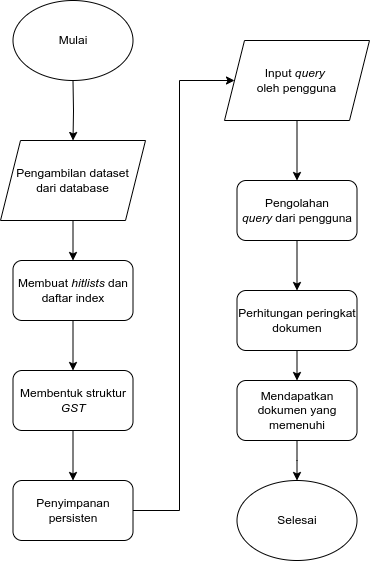
\includegraphics[width=0.6\textwidth]{gambar/flowchart_awal}
  \caption{Flowchart tahapan penelitian modul \textit{indexing}}
\end{figure}

Data utama yang diperlukan oleh modul \textit{indexing} dari database adalah
teks yang berisi bagian informasi inti dari halaman tersebut. Umumnya, sebuah
halaman web memiliki banyak teks di luar informasi inti yang tidak diperlukan.
Oleh karena itu, ditetapkan bahwa modul \textit{indexing} hanya akan mengambil
bagian paragraf dari halaman web. Untuk mengidentifikasi sebuah paragraf, cukup
dengan mencari \textit{tag} HTML yang sesuai (\textit{<p>}).

Walaupun sudah menspesifikasikan \textit{tag} tertentu yang akan digunakan, pada
praktiknya sering ditemukan penggunaan \textit{tag} paragraf di luar informasi
inti halaman web. Selain itu, seringkali ditemukan paragraf yang memiliki
beberapa simbol yang tidak diperlukan seperti karakter \textit{newline}. Untuk
memastikan bahwa modul \textit{indexing} hanya akan membaca paragraf inti saja,
diperlukan \textit{filter} khusus untuk menghindari masuknya informasi yang
tidak diperlukan. Parameter dari penentuan informasi ini cukup beragam, dan akan
diatur sedemikian rupa pada masa pengujian.

Pada kode program mesin pencari yang telah ada saat ini, paragraf yang disimpan
masih memiliki banyak informasi yang tidak diperlukan. Untuk memudahkan
implementasi modul \textit{indexing}, maka proses \textit{filtering} akan
dilakukan pada kode mesin pencari di bagian ekstraksi informasi dari halaman
web. Akan dibuat sebuah table baru yang berisi paragraf inti saja.

\section{Konstruksi Index}

Sebelum proses \textit{indexing} dilakukan, diperlukan sebuah
\textit{hash table} pada memori. \textit{Hash table} digunakan dengan tujuan
untuk menyimpan kata secara unik dalam dokumen. Jika nantinya ditemukan lebih
dari satu kali kemunculan kata dalam dokumen yang sama, \textit{hash table}
dapat melakukan penambahan kepada \textit{value} dari kata tersebut, dan
membentuk suatu rangkaian seperti \textit{linked list}.

% baca webpage dan ekstrak metadata
Proses \textit{indexing} dimulai dengan mengambil seluruh daftar paragraf yang
tersimpan pada database yang diurutkan berdasarkan \textit{docID}. Kemudian,
setiap paragraf akan dipecah berdasarkan karakter spasi menjadi sebuah array
berisi kata. Setiap kata lalu disimpan dalam sebuah hit bersama dengan informasi
tambahan yang ada pada paragraf.

\begin{algorithm}[H]
  \caption{Algoritma pembuatan index (\cite{brin1998google})}\label{alg:index}
  \begin{algorithmic}
    \State $hitData \gets \Call{HitData}{false}$ \Comment{Inisiasi \textit{hash table}}
    \State $docMap \gets [..]$

    \item[] % line skip

    \State $docs[..] \gets \Call{GetDocs}$
    \For{$doc \in \mathcal{} docs[..]$}
      \State $paragraphs[..] \gets \Call{GetParagraphs}{$doc$}$
      \For{$paragraph \in \mathcal{} paragraphs[..]$}
        \State $words[..] \gets \Call{SplitWords}{$$paragraph$$}$

        \item[] % line skip

        \For{$word \in \mathcal{} words[..]$}
          \State $\Call{StoreHit}{$$hitData, word$$}$
        \EndFor

        \item[] % line skip

          \State $\Call{docMap}{$doc$} \gets hitData$
      \EndFor
    \EndFor
  \end{algorithmic}
\end{algorithm}

Dari proses ekstraksi kosakata beserta data tambahannya, akan didapatkan
\textit{forward index} berupa daftar \textit{hit} dari dokumen. Daftar
\textit{hit} kemudian didistribusikan ke tempat penyimpanan.

% sorting forward index jadi inverted
Untuk melakukan konversi \textit{forward index} menjadi \textit{inverted index},
dilakukan proses \textit{sorting} pada \textit{forward index}. \textit{Sorting}
dilakukan berdasarkan \textit{id} dari kosakata, kemudian dilanjutkan dengan
\textit{id} dari dokumen, dan diakhiri dengan posisi kata pada dokumen. Hasil
dari proses \textit{sorting} disimpan kembali ke tempat penyimpanan dengan
kondisi sudah menjadi \textit{inverted index}.

\begin{algorithm}[H]
  \caption{Operasi \textit{sorting} pada \textit{hitlist} (\cite{brin1998google})}\label{alg:insert}
  \begin{algorithmic}
    \Function{SortHitlist}{$H$}
      \State $sorted \gets false$
      \State $i \gets 0$

      \item[] % line skip

        \Do
          \If{$i = \Call{Len}{H} - 1$}
            \If{$sorted = true$}
              \State $break$
            \Else
              \State $i \gets 0$
            \EndIf
          \EndIf

          \item[] % line skip

          \State $tempHit \gets H[i]$

          \item[] % line skip

          \If{$H[i].text > H[i+1].text$ OR
          \newline \hspace*{3.8em}$H[i].docID > H[i+1].docID$ OR
          \newline \hspace*{3.8em}$H[i].oset > H[i+1].oset$}
            \State $H[i] \gets H[i+1]$
            \State $H[i+1] \gets tempHit$
          \EndIf

          \item[] % line skip

          \State $i \gets i+1$
        \doWhile{$sorted = false$}

        \item[] % line skip

      \State \Return
    \EndFunction
  \end{algorithmic}
\end{algorithm}

\section{Daftar kata umum}

Untuk meningkatkan kualitas hasil pencarian, maka skema pencarian perlu
mengabaikan kata-kata yang bersifat umum. Dari hal tersebut, perlu di dapatkan
daftar kata umum dari daftar kosakata yang telah dibuat oleh modul
\textit{indexing}. Metode yang penulis gunakan untuk mendapatkan kata umum
adalah dengan melakukan \textit{sorting} terhadap seluruh daftar kosakata
berdasarkan tingkat kemunculannya secara global. Kemudian, dengan menggunakan
batasan tertentu, akan diambil sebagian persen dari kata terbanyak yang ada.

Sebagai langkah awal, penulis berencana untuk mengambil sebanyak 1\% kata
teratas sebagai kata umum. Nilai tersebut kemudian akan diatur ulang berdasarkan
hasil \textit{user testing}.

\section{Metode Pemeringkatan}

Dari hasil rangkaian \textit{hit} yang didapatkan, perlu dilakukan beberapa
operasi untuk mendapatkan urutan hasil dokumen yang paling sesuai. Hasil
peringkat yang didapatkan dilakukan berdasarkan dua faktor berikut

\begin{itemize}
  \item{\textit{Word distance ($\gamma$)}, yaitu jarak kata yang memenuhi query}
  \item{\textit{Word similarity ($\beta$)}, yaitu kemunculan hasil yang memenuhi beberapa
    bagian dari query}
\end{itemize}

\subsection{\textit{Word distance ($\gamma$)}}

Perhitungan \textit{word distance} digunakan untuk melakukan validasi terhadap
urutan kata yang muncul pada dokumen. Urutan dari kata berpengaruh terhadap
maksud dari query. Selain itu, jarak yang terlalu jauh antara kata yang
ditemukan dapat mengurangi relevansi informasi.

Untuk membandingkan jarak kata, seluruh kata pada query perlu diberikan urutan
yang sesuai dengan menggunakan angka terlebih dahulu. Setelah \textit{hitlist}
didapatkan, posisi dari kata yang ditemukan akan dikurangi dengan posisi asli
pada query. Nilai dari dokumen bisa didapatkan dengan rumus

% TODO Revisi rumusnya dikit
\begin{equation}
  \gamma = \left(\sum_{n = 1}^{N} |L_n - \acute{L_n}|\right) - (L_1 - \acute{L_1}) \times N
  \label{eq:word_distance}
\end{equation}

di mana

\begin{conditions}
  N & Jumlah kata pada query \\
  L_n & Posisi awal kata ke-$n$ pada query \\
  \acute{L_n} & Posisi kata ke-$n$ pada query di dokumen
\end{conditions}

Ketika urutan kata pada dokumen meiliki nilai $\gamma = 0$, maka dokumen 
memenuhi kondisi \textit{exact match}. Pada kondisi tersebut, dokumen akan 
mendapatkan peringkat berdasarkan jumlah kemunculan \textit{exact match}. Sementara 
jika nilai $\gamma \not = 0$, maka dokumen akan mendapatkan peringkat 
berdasarkan rumus berikut 

\begin{equation}
  D = \frac{n}{N} + (\frac{n}{N} \times \frac{1}{G} \times K)
  \label{eq:word_distance_partial}
\end{equation}

di mana

\begin{conditions}
  n & Jumlah \textit{match} pada dokumen \\
  N & Jumlah kata pada query \\
  G & Faktor kemunculan terhadap nilai $\gamma$ \\
  K & Jumlah kemunculan \textit{partial match}
\end{conditions}

Apabila dalam suatu dokumen, terdapat berbagai kondisi \textit{match} dengan 
nilai $\gamma$ yang berbeda-beda, maka akan dipilih kondisi \textit{match} 
dengan nilai $\gamma$ paling rendah untuk merepresentasikan nilai dokumen.

\subsection{\textit{Word similarity ($\beta$)}}

\textit{Word similarity} menilai suatu kata berdasarkan kemiripannya dari kata
pada query. Untuk membandingkan apakah suatu kata memiliki makna atau maksud
yang sama dengan kata lainnya, akan digunakan \textit{Jaccard distance}.
Perbandingan akan dilakukan berdasarkan hasil kombinasi pada seluruh karakter
yang ada pada kosakata untuk membuat pasangan dua huruf.

Karena \textit{Jaccard distance} mengukur nilai ketidakmiripan dari dua model,
maka tinggi nilai $\beta$ maka nilai dokumen akan makin rendah. Dari detail
tersebut, didapatkan rumus

\begin{equation}
  \beta = 1 - \frac{m}{M}
  \label{eq:word_similarity}
\end{equation}

di mana

\begin{conditions}
  m & Jumlah pasangan dua huruf berurutan yang ada pada kata \\
  M & Jumlah kemungkinan seluruh pasangan dua huruf berurutan yang mungkin
      dibentuk \\
\end{conditions}

% TODO Ada plan untuk menggunakan cache (ini ngide aje)
Karena proses perhitungannya yang cukup kompleks, metode pemeringkatan ini hanya
digunakan ketika nilai dari \textit{word distance} bernilai kurang dari satu.

\section{Modifikasi Arsitektur \textit{Telusuri}}

\begin{figure}[H]
  \centering{}
	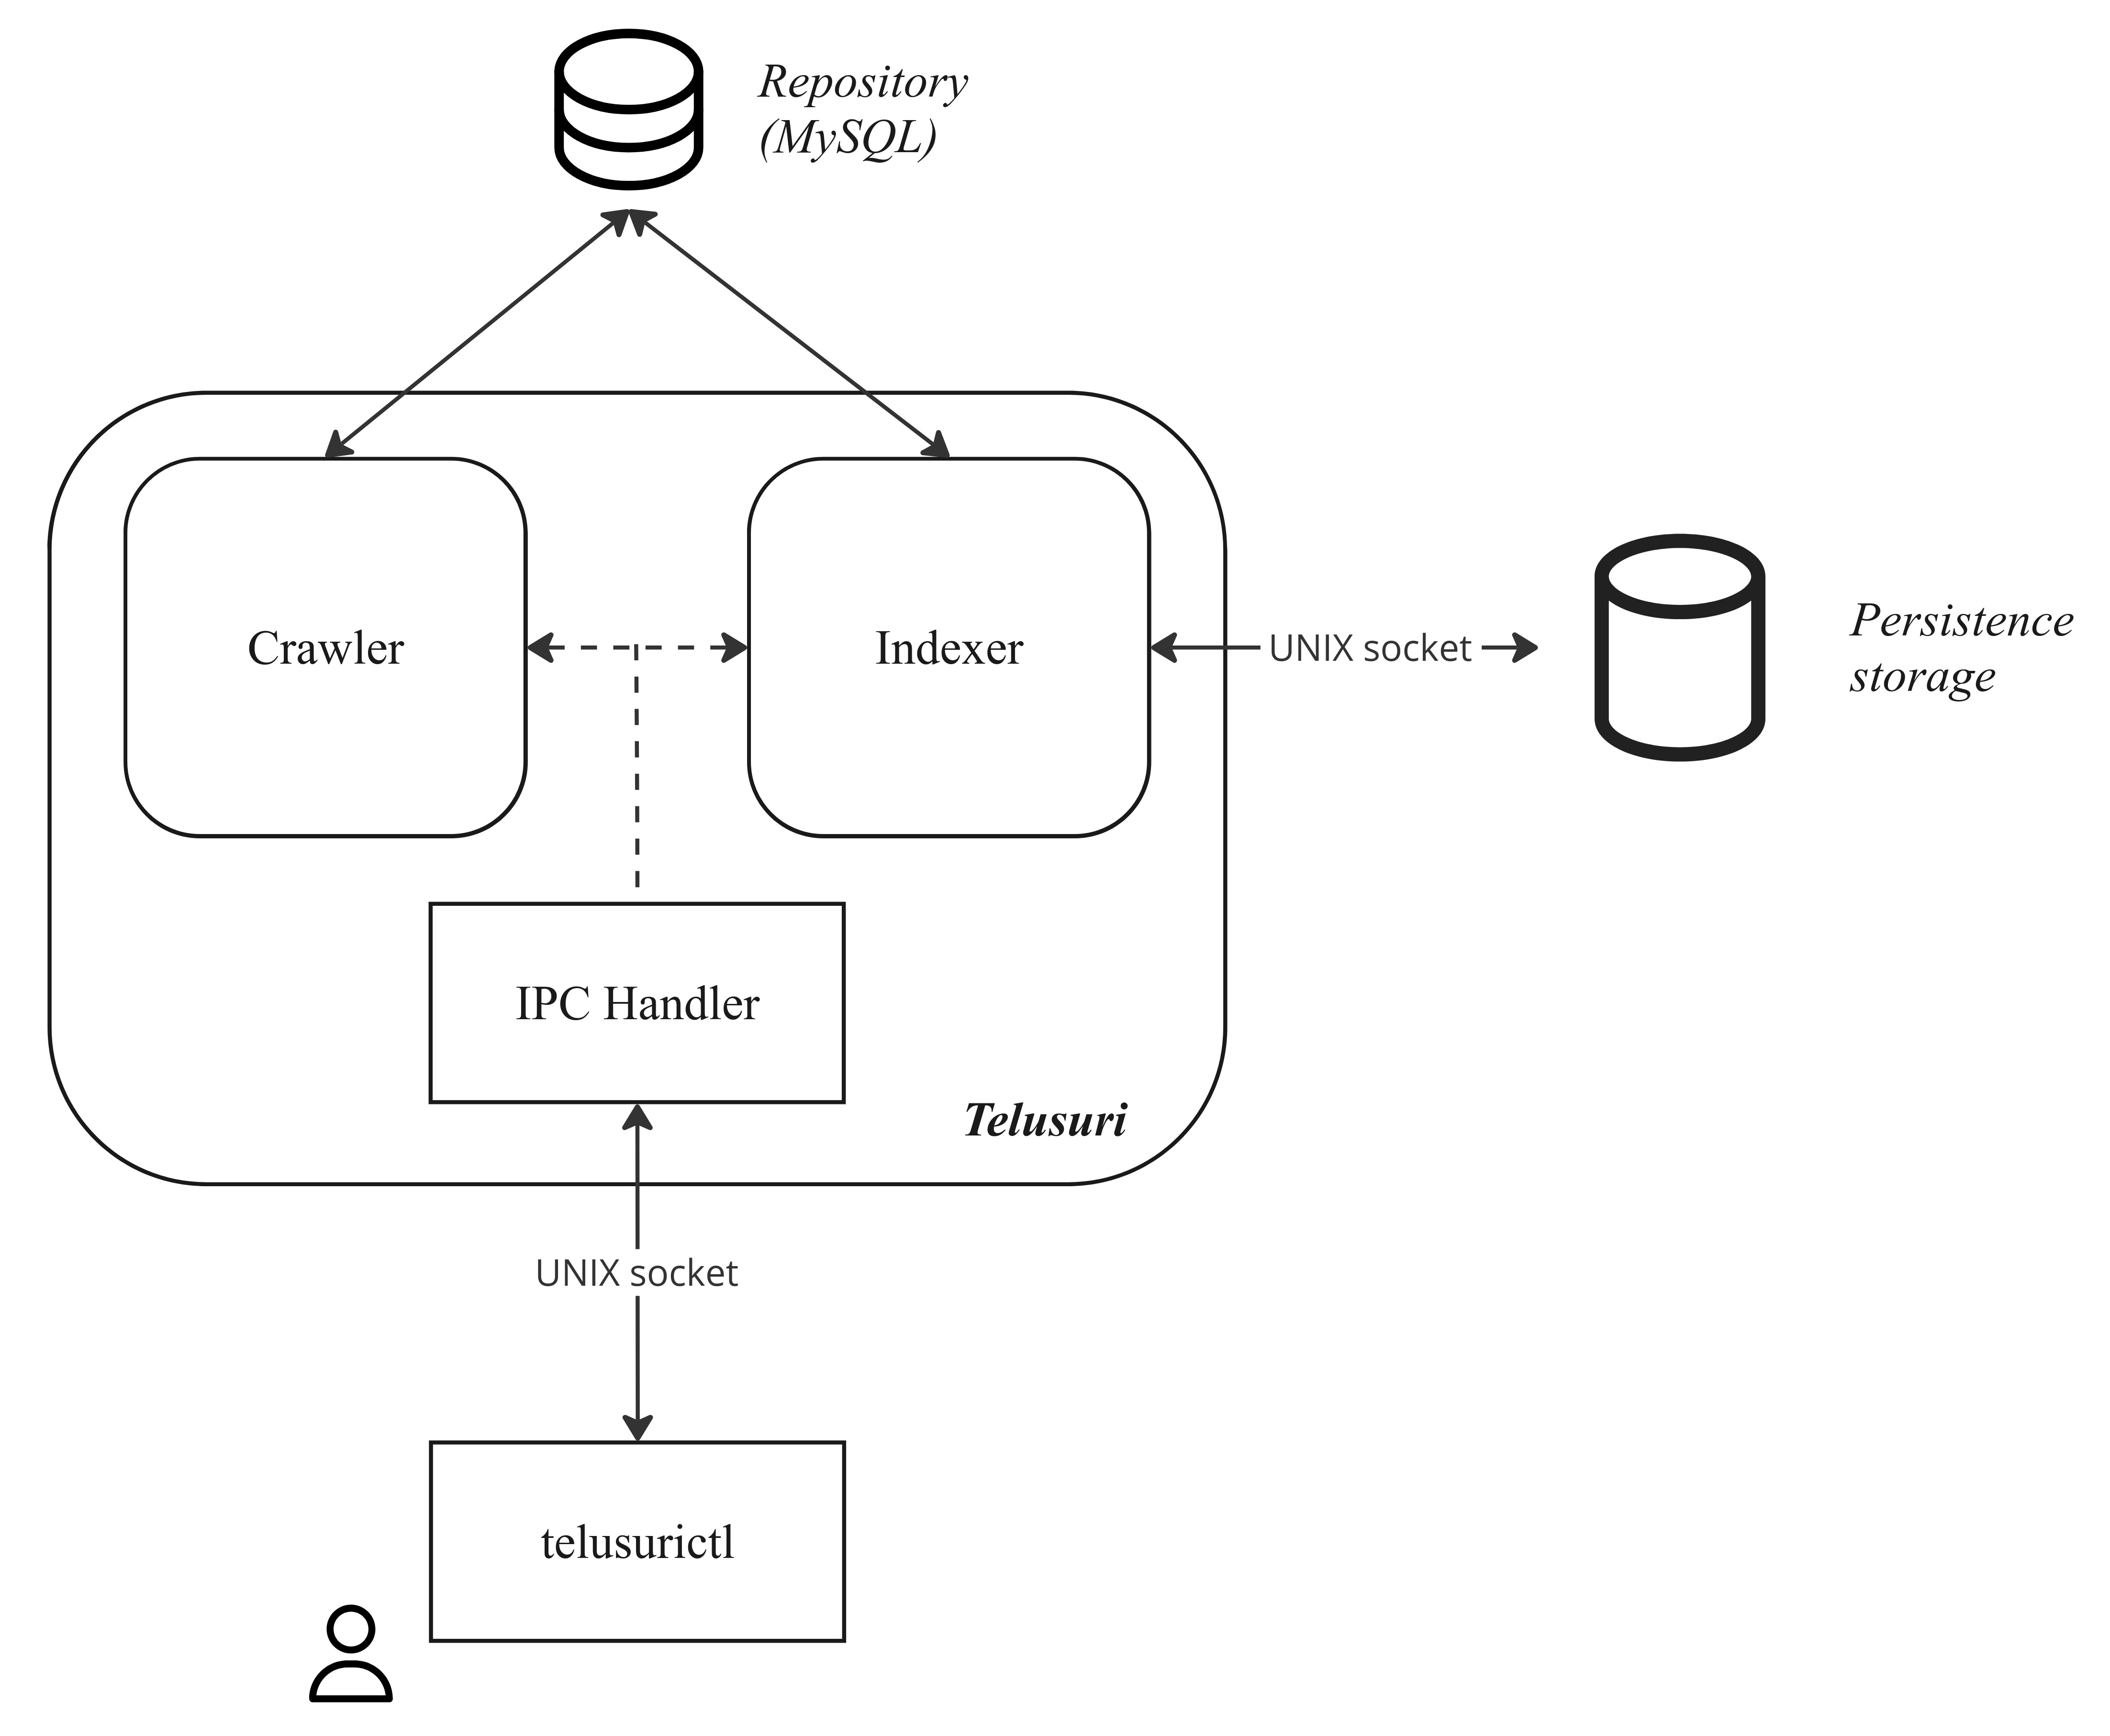
\includegraphics[width=0.8\textwidth]{gambar/arsitektur_baru}
  \caption{Revisi arsitektur \textit{Telusuri}}
\end{figure}

Dari arsitektur \textit{Telusuri} yang sudah ada saat ini, terdapat beberapa 
perubahan yang perlu dilakukan untuk mengintegrasikan modul \textit{indexing}
ini.

\begin{itemize}
  \item{\textit{Telusuri} dibagi menjadi dua mode \textit{runtime}, yaitu 
    \textit{crawling} dan \textit{indexing}.}
  \item{Kontrol terhadap berjalannya \textit{Telusuri} akan dikendalikan oleh 
    aplikasi \textit{command-line}, yaitu \textit{telusurictl}. \textit{telusurictl} 
    akan berkomunikasi dengan \textit{Telusuri} melalui sebuah metode komunikasi 
    antar proses. Untuk metode komunikasi akan digunakan, ditentukan untuk 
    menggunakan \textit{UNIX domain socket} dengan alasan didukung secara 
    langsung oleh sistem operasi yang digunakan (Linux) dan bersifat
    \textit{language-agnostic} sehingga mudah untuk dikembangkan kedepannya.}
  \item{Terdapat modul database primitif yang berperan sebagai \textit{persistent 
    storage} untuk \textit{hitlists} yang telah dibuat oleh modul \textit{indexing}.
    Modul database ini berjalan sebagai proses terpisah, tetapi tetap dalam satu 
    mesin yang sama. Modul akan memberikan \textit{hitlists} sesuai dengan 
    rentang yang diminta oleh modul \textit{indexing}. Untuk komunikasi antar 
    modul, akan digunakan \textit{UNIX domain socket}.}
\end{itemize} 

\section{Skema Pencarian}

Untuk mendapatkan informasi pencarian berdasarkan input teks dari pengguna,
diperlukan beberapa informasi tertentu yang bisa didapatkan dengan cara mengolah 
informasi yang ada pada teks tersebut. Objek \textit{UserQuery} digunakan untuk 
mengakomodasi kebutuhan itu.

\begin{figure}[H]
  \centering{}
	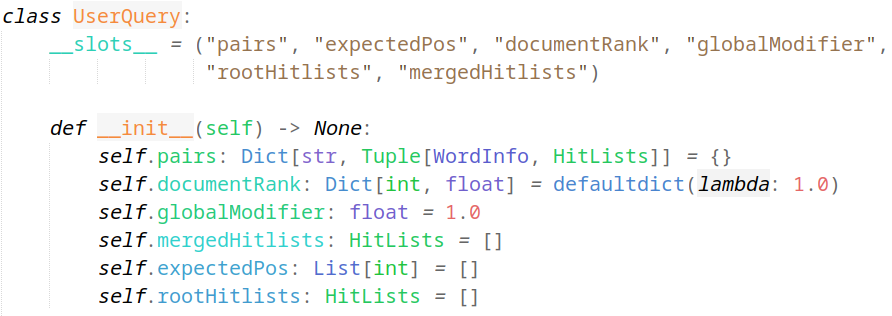
\includegraphics[width=0.8\textwidth]{gambar/struktur_userquery}
  \caption{Struktur objek \textit{UserQuery}}
\end{figure}

% Parsing query
Berdasarkan input query yang diberikan oleh pengguna, query dipecah menjadi
potongan kata dan ditetapkan beberapa informasi tambahan bedasarkan 
karakteristik dari masing-masing kata. Informasi tersebut adalah posisi kata 
dalam teks input, apakah kata tersebut termasuk kata umum dan apakah kata 
tersebut termasuk kapital. Ketiga informasi ini akan disimpan sebagai
\textit{WordInfo} yang ada pada objek \textit{UserQuery}.

\begin{figure}[H]
  \centering{}
	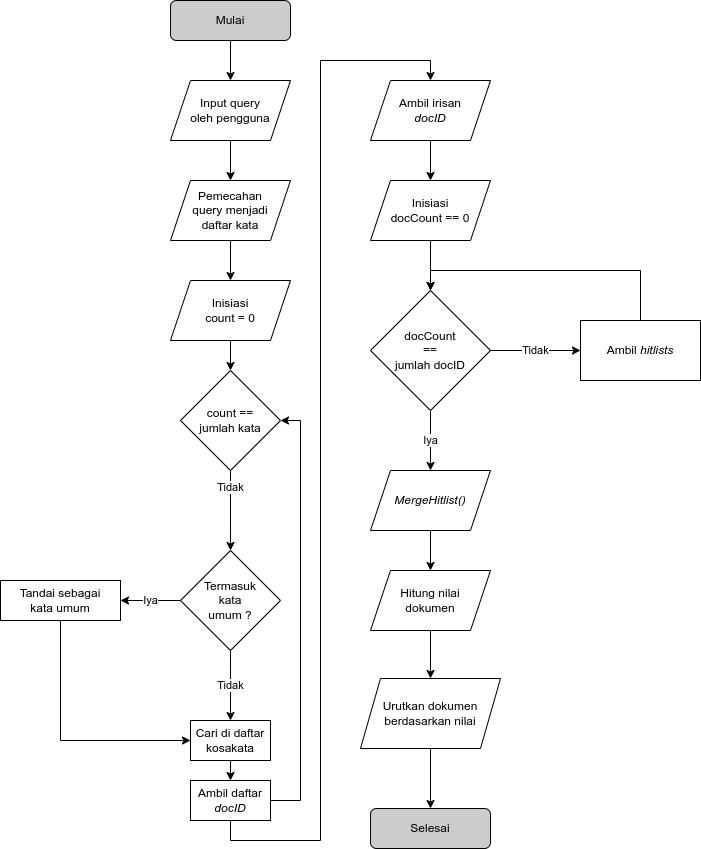
\includegraphics[width=0.85\textwidth]{gambar/flowchart_pencarian}
  \caption{Flowchart pengolahan masukan query}
\end{figure}

Untuk setiap kosakata pada daftar kosakata yang sesuai dengan kosakata pada
query, akan di dapatkan rangkaian data berupa \textit{id} dari dokumen tempat
kosakata tersebut, total jumlah \textit{hit} pada dokumen serta seluruh daftar
\textit{hit} yang berhubungan dengan kosakata pada dokumen.

\begin{figure}[H]
  \centering{}
	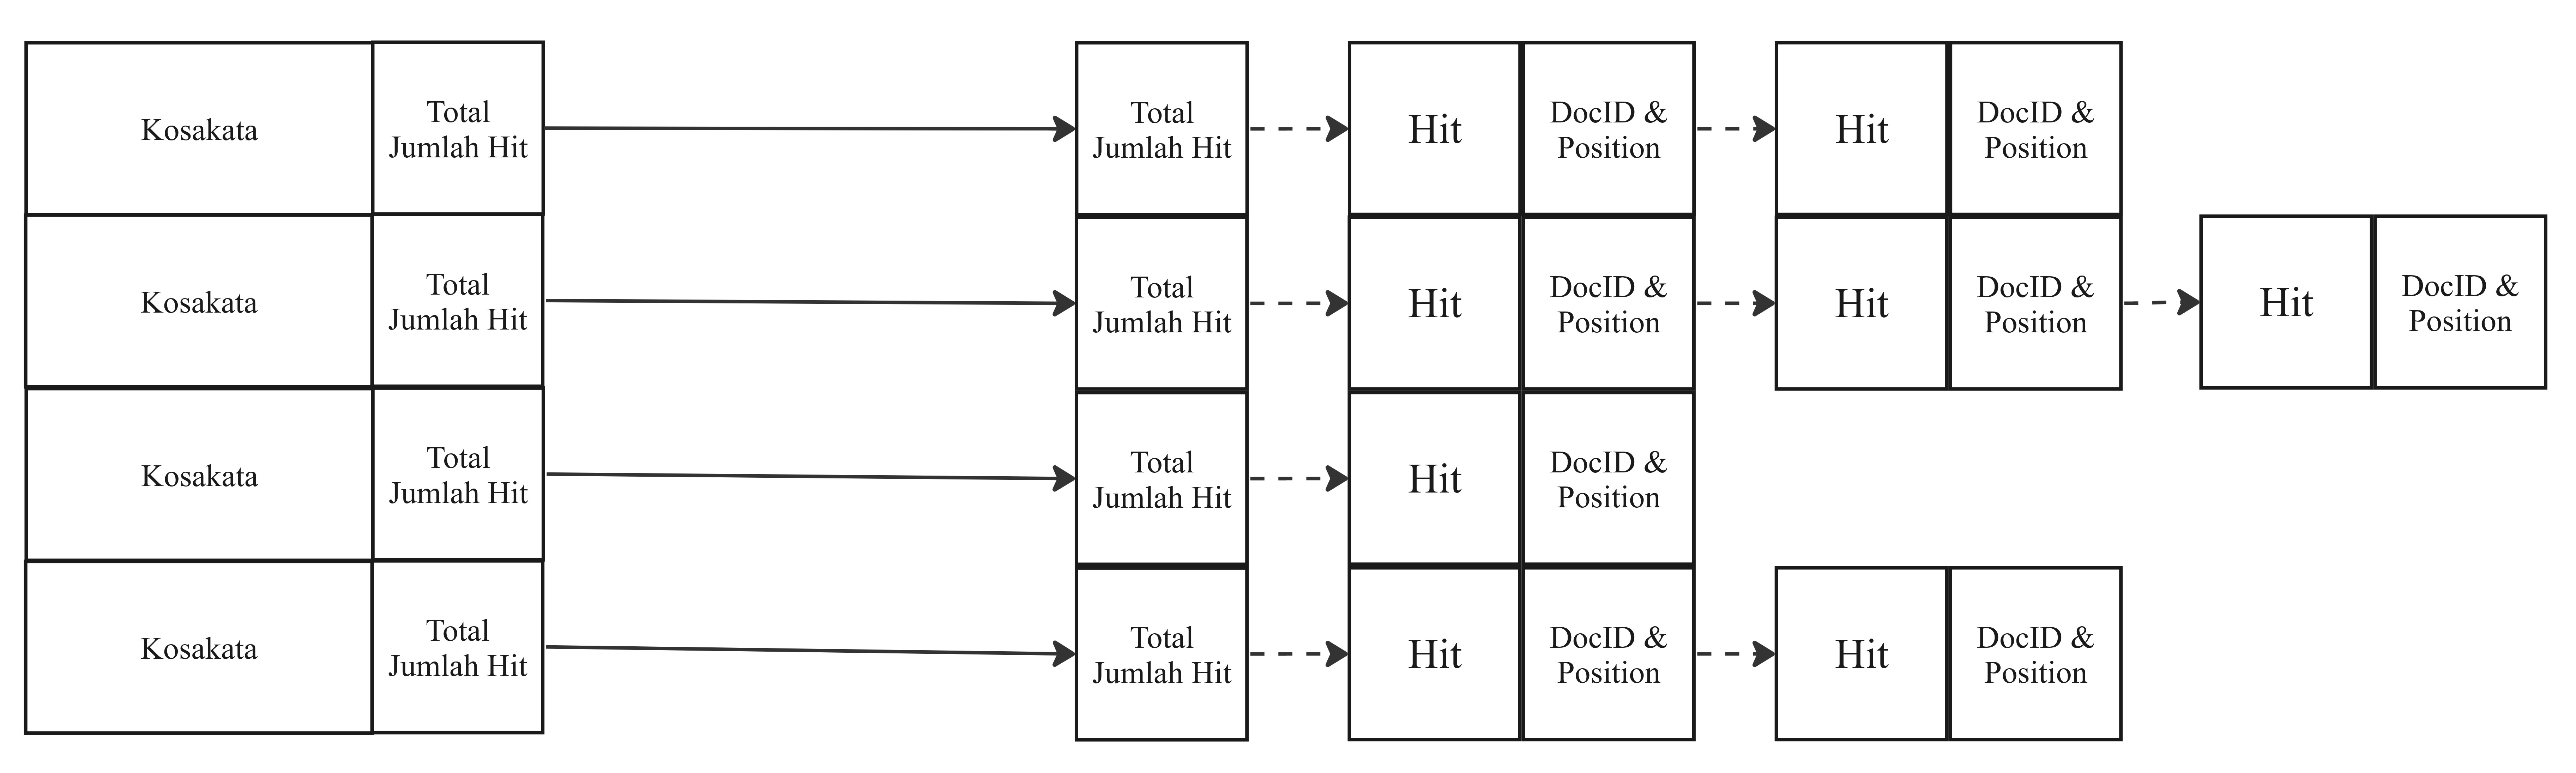
\includegraphics[width=1\textwidth]{gambar/struktur_data_gambar}
  \caption{Ilustrasi hubungan struktur data}
\end{figure}

\begin{figure}[H]
  \centering{}
	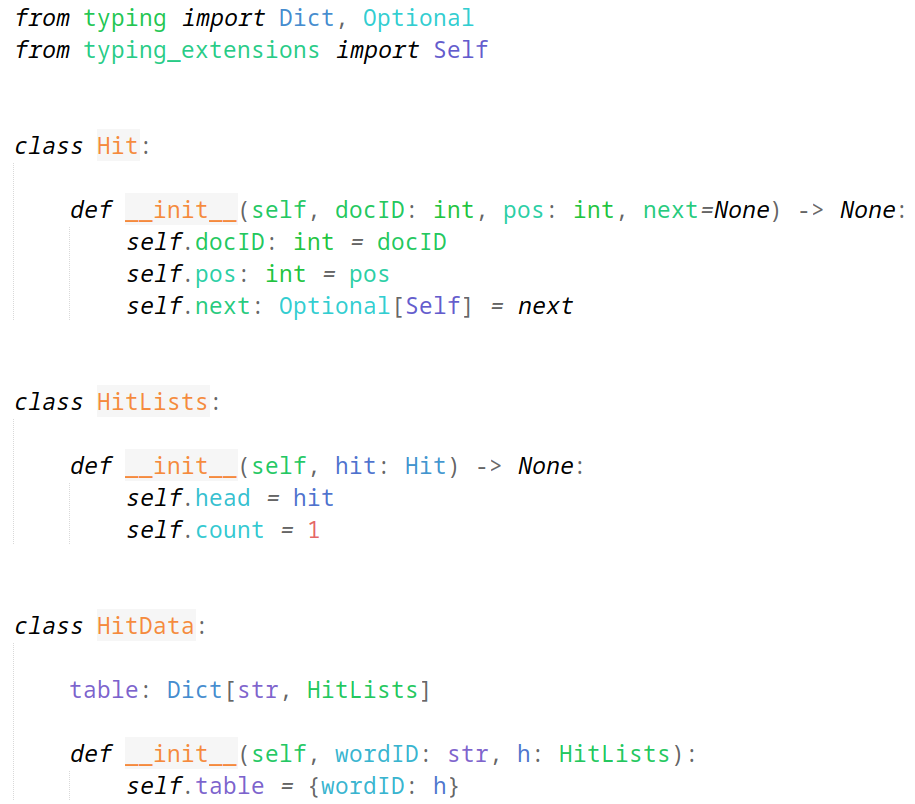
\includegraphics[width=0.9\textwidth]{gambar/struktur_data_python}
  \caption{Penulisan struktur data pada \textit{Python}}
\end{figure}

Untuk setiap daftar \textit{hit} yang didapatkan, dilakukan \textit{merging}
sehingga tersisa dokumen yang memenuhi query.

\begin{algorithm}[H]
  \label{alg:merge}
  \caption{Operasi \textit{merging} pada seluruh \textit{hitlists} (\cite{brin1998google})}
  \begin{algorithmic}
    \Function{MergeHitlist}{$p1$, $p2$}
    \State $M \gets [..]$
    \While{$p1 \not = nil$ AND $p2 \not = nil$}
      % TODO Handle multiline
      \If{$p1.docID = p2.docID$} \Comment{Cek kesamaan \textit{docID}}
        \If{$-(p1.oset - p2.oset)$ = 1} \Comment{Cek selisih offset}
          \State \Call{Append}{$M$, $p1$}
        \EndIf
      \EndIf
      \State $p1 \gets \Call{next}{$p1$}$
      \State $p2 \gets \Call{next}{$p2$}$
    \EndWhile{}
    \State \Return $M$
    \EndFunction

    \item[] % line skip

    \State $H \gets [..]$
    \State $W \gets \Call{ParseQuery}{query}$ \Comment{Pecah query menjadi
    daftar kata}
    \For{$w \in \mathcal{} W$}
      \State $h \gets \Call{GetHitlist}{w}$
      \If{$h = nil$}
        \State continue
      \EndIf
      \State \Call{Append}{H, h}
    \EndFor

    \item[] % line skip

    \State $i \gets 0$
    \While{$i \not = \Call{Len}{H}$}
      \State $H[0] = \Call{MergeHitlist}{$H[0]$, $H[i]$}$
      \State $i \gets i + 1$
    \EndWhile

    \item[] % line skip

    \State $result \gets \Call{GetResult}{H[0]}$
  \end{algorithmic}
\end{algorithm}

\section{Alat dan Bahan Penelitian}

Pada penelitian ini, terdapat beberapa alat yang digunakan sebagai penunjang
dalam pembuatan modul \textit{indexing} dengan rincian sebagai berikut:

\begin{itemize}
  \item{Laptop dengan konfigurasi Intel Core i7-8650U, 32GB RAM)}
  \item{Sistem operasi \textit{Linux}}
  \item{\textit{Neovim} sebagai \textit{code editor}}
  \item{Database \textit{MySQL} versin $8.0.31$}
  \item{\textit{Podman} untuk menjalankan database \textit{MySQL}}
  \item{\textit{Python 3.8}}
\end{itemize}

\section{Tahapan Pengembangan}

\subsection{Meningkatkan kemampuan modul \textit{indexing} saat ini}

Pencarian akan dilakukan secara sekuensial terhadap daftar index yang telah
dihasilkan oleh modul \textit{indexing}. Sebagai pembanding, modul dari
penelitian ini akan digabungkan dengan modul \textit{indexing} yang sudah ada 
saat ini (\cite{zaidan2023gst}).

Hasil penelitian tersebut menghasilkan modul \textit{indexing} dengan bentuk
\textit{Generalized Suffix Tree (GST)}. Penggunaan modul \textit{GST} bertujuan
untuk menghindari proses iterasi daftar kosakata yang bisa memakan waktu yang
cukup lama. Modul \textit{GST} dapat langsung memberikan hasil berupa dokumen
tempat kata tersebut berada. Dengan demikian, modul index pada penelitian ini
hanya perlu menunjukkan lokasi kata pada dokumen melalui informasi yang ada
pada \textit{hit}. Selain itu, penggunaan \textit{GST} juga dapat melakukan
koreksi terhadap adanya \textit{typo} pada query yang diberikan oleh pengguna.

Untuk mendukung integrasi dengan modul \textit{GST}, diperlukan pemetaan dari
dokumen ke \textit{hitlists} yang sesuai. Oleh karena itu, akan dilakukan 
modifikasi pada \ref{alg:index} untuk menambahkan pemetaan dokumen ke
\textit{hitlists} yang terbentuk.

\begin{figure}[H]
  \centering{}
	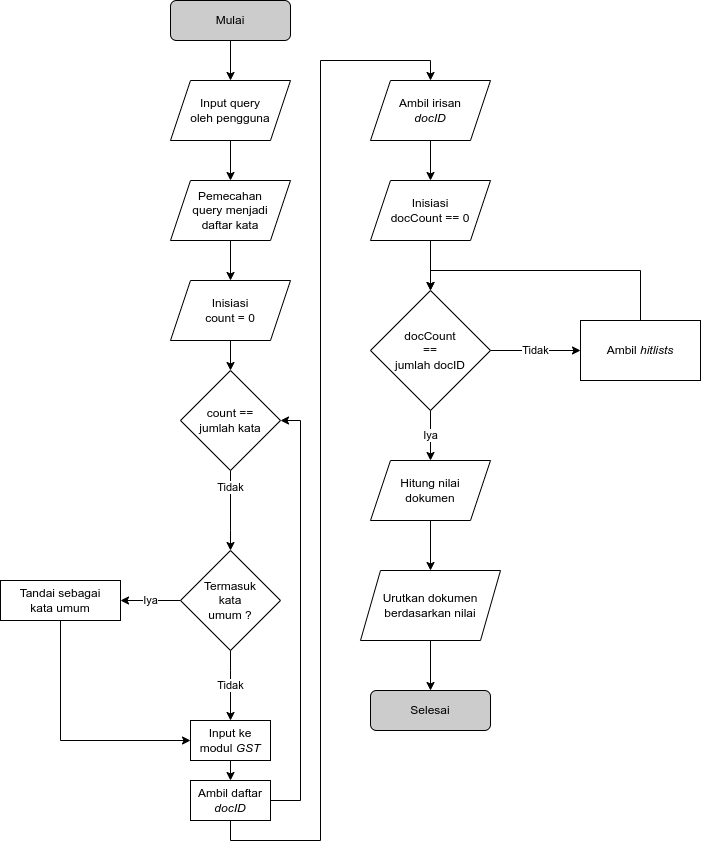
\includegraphics[width=0.8\textwidth]{gambar/flowchart_pencarian_gst}
  \caption{Flowchart pengolahan masukan query dengan modul \textit{GST}}
\end{figure}

Integrasi dilakukan dengan modul \textit{GST} yang telah dibuat pada penelitian 
sebelumnya, dengan beberapa perbaikan dan penambahan fungsi pembantu untuk 
mempermudah integrasi.

\subsection{Rancangan Eksperimen}

\begin{enumerate}
  \item{Skenario pertama (Pencarian degnan iterasi daftar kosakata)}
    \begin{itemize}
      \item{Pencatatan waktu akan mulai mencatat}
      \item{\textit{Tester} memberikan sebuah query ke dalam mesin pencari}
      \item{Sistem memecah kata berdasarkan spasi}
      \item{Sistem melakukan iterasi pada daftar kosakata untuk mencari kata 
        yang sesuai dengan query}
      \item{Sistem melakukan pencarian pada kata dengan mencari pada daftar 
        kosakata}
      \item{Sistem menggabungkan seluruh hasil pencarian per kata}
      \item{Sistem melakukan pemeringkatan hasil}
      \item{Sistem mengembalikan daftar dokumen hasil pencarian yang diurutkan
        berdasarkan hasil pemeringkatan}
      \item{Pencatatan waktu berhenti mencatat}
      \item{\textit{Tester} memberikan penilaian terhadap relevansi dari hasil
        pencarian}
      \item{Hasil perhitungan waktu akan dibandingkan dengan skenario lain}
    \end{itemize}
  \item{Skenario kedua (Pencarian dengan integrasi modul GST)}
    \begin{itemize}
      \item{Pencatatan waktu akan mulai mencatat}
      \item{\textit{Tester} memberikan sebuah query ke dalam mesin pencari}
      \item{Sistem memecah kata berdasarkan spasi}
      \item{Sistem melakukan input kata ke modul \textit{GST} dan mendapatkan 
        output berupa hasil pencarian}
      \item{Sistem menggabungkan seluruh hasil pencarian per kata}
      \item{Sistem melakukan pemeringkatan hasil}
      \item{Sistem mengembalikan daftar dokumen hasil pencarian yang diurutkan
        berdasarkan hasil pemeringkatan}
      \item{Pencatatan waktu berhenti mencatat}
      \item{\textit{Tester} memberikan penilaian terhadap relevansi dari hasil
        pencarian}
      \item{Hasil perhitungan waktu akan dibandingkan dengan skenario lain}
    \end{itemize}
\end{enumerate}
